\documentclass[12pt]{article}
\usepackage[utf8]{inputenc}
\usepackage{acronym}
\usepackage{amsmath}
\usepackage{amsfonts}
\usepackage{amssymb}
\usepackage{booktabs}
\usepackage{braket}
\usepackage{changepage}
\usepackage{enumitem}
\usepackage{fancyhdr}
\usepackage{graphicx}
\usepackage{geometry}
\usepackage[none]{hyphenat}
\usepackage{lipsum}
\usepackage{multicol}
\usepackage[numbers]{natbib}
\usepackage{parskip}
\usepackage{subcaption}
\usepackage{tabularx}
\geometry{a4paper, margin=1in}
\setlength{\columnsep}{0.7cm}
\newcommand{\vctr}[1]{\ensuremath{\mathbf{#1}}}
\newcommand{\vctrg}[1]{\mbox{\boldmath{$#1$}}}
\newcommand{\unitr}[1]{\ensuremath{\mathbf{\hat{#1}}}}
\newcommand{\depar}[2]{\ensuremath{\frac{\partial#1}{\partial#2}}}
\newcommand{\depars}[2]{\ensuremath{\frac{\partial^{2}#1}{\partial#2^{2}}}}
\newcommand{\perme}{\ensuremath{\epsilon_{0}}}
\newcommand{\permm}{\ensuremath{\mu_{0}}}
\newcommand{\unitrg}[1]{\mbox{\boldmath{$\hat{#1}$}}}

\title{Heat Transfer in Radial Direction in Fuel Elements and Reactor Core}
\author{Md. Ariful Islam \\ Email: islamm65@mcmaster.ca \\ Department of Engineering Physics, McMaster University}
\date{}     

\begin{document}

% Header & Footer Stuff
\pagestyle{fancy}
\fancyhf{}                       % Clear default headers and footers
\fancyhead[L]{Heat Transfer in Reactor Core} 
\fancyhead[R]{\today}           
\renewcommand{\headrulewidth}{0.4pt} 
\fancyfoot[C]{\thepage}

\maketitle
\thispagestyle{fancy}

\section*{\centering Abstract} 

\textit{Heat transfer in nuclear fuel elements plays a crucial role in reactor thermal performance and safety. This assignment explores the mechanisms governing radial heat dissipation, including conduction within the fuel pellet, cladding, fuel-cladding gap, and convective cooling by the coolant. Key material properties, such as thermal conductivities of the fuel and cladding, are discussed to assess their impact on the temperature distribution. The mathematical formulation of radial heat conduction is presented, including analytical and numerical approaches for temperature profile evaluation. Modeling techniques, such as Finite Difference (FDM), Finite Element (FEM), and Computational Fluid Dynamics (CFD) methods, are discussed for accurate heat transfer simulations. The study concludes with recommendations for advanced materials and improved modeling techniques to enhance reactor design and operational safety.}

%% -----------------------
%%      Introduction
%% -----------------------
\begin{multicols}{2}

\section{Introduction}
Efficient heat transfer in nuclear reactors is essential for maintaining structural integrity, optimizing performance, and ensuring operational safety. Among the various heat transfer pathways, radial heat dissipation in fuel elements plays a critical role in regulating fuel temperature and preventing excessive thermal stresses. The ability of a reactor to efficiently remove heat from the fuel to the coolant depends on multiple factors, including fuel composition, cladding properties, and thermal resistance at various interfaces.

In nuclear fuel elements, heat is primarily generated by fission reactions and must be transported radially from the fuel to the outer surface, where it is transferred to the coolant. This process involves conduction within the fuel pellet and cladding, and convective heat removal by the coolant. This assignment examines the key physical phenomena governing radial heat transfer in reactor cores, along with a review of material properties affecting heat conduction. Mathematical models and evaluation techniques, including analytical and numerical methods, are discussed. Additionally, advanced modeling approaches such as Finite Difference (FDM), Finite Element (FEM), and Computational Fluid Dynamics (CFD) methods are explored to enhance predictive capabilities. Finally, the study presents recommendations for improved thermal management strategies in nuclear reactors.

\end{multicols}

%% ----------------------------------------------
%%      Radial Heat Transfer in Fuel Elements
%% ----------------------------------------------
\begin{multicols}{2}
\section{Radial Heat Transfer in Fuel Elements}

Radial heat transfer in nuclear fuel elements is critical for reactor safety. It primarily occurs through conduction within the fuel and cladding, followed by convective heat transfer to the coolant. The thermal performance is influenced by factors such as material properties, power density, and burnup effects.

\begin{itemize}
    \item \textbf{Heat Transfer Mechanisms}
    \begin{enumerate}[itemindent=1cm]
        \item \textit{Conduction in Fuel and Cladding} 
        \item[] Heat generated in the fuel pellet is transferred radially through conduction. The thermal conductivity of $(UO_{2})$, the most common fuel, decreases with temperature and burnup due to fission product accumulation and radiation damage \cite{osti_1035151} as shown in Figure \ref{fig:fig_1}. The cladding, typically zirconium-based, also undergoes irradiation-induced changes affecting heat transfer.
        \item \textit{Convection in Coolant}
        \item[] The cladding surface transfers heat to the coolant via convection. The effectiveness depends on the coolant properties, flow rate, and phase conditions. A higher convective heat transfer coefficient enhances cooling and reduces cladding surface temperatures. 
    \end{enumerate}
    \item \textbf{Effects of Burnup on Radial Heat Transfer}
    \begin{itemize}
        \item \textbf{Fuel Pellet Degradation:} Burnup reduces fuel thermal conductivity due to radiation damage and fission product buildup.
        \item \textbf{Cladding Evolution:} Fast neutron irradiation causes embrittlement, oxidation, and creep, reducing heat transfer efficiency over time.
    \end{itemize}
\end{itemize}

\end{multicols}

\begin{figure}
    \centering
    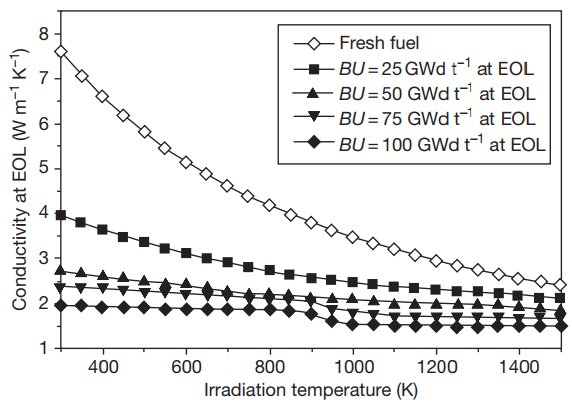
\includegraphics[width=0.7\linewidth]{figs/Thermal-conductivity-of-UO2-as-function-of-burn-up.png}
    \caption{Thermal conductivity of $(UO_{2})$ as function of burnup}
    \label{fig:fig_1}
\end{figure}

%% ----------------------------------------------
%% Review of Materials and Thermal Properties
%% ----------------------------------------------
\begin{multicols}{2}

\section{Review of Materials and Thermal Properties}

The efficiency of radial heat transfer in a nuclear reactor is strongly influenced by the thermal properties of fuel, cladding, and coolant.

\begin{itemize}[leftmargin=0pt]
    \item[] \textbf{Fuel Materials and Thermal Conductivity}

    Uranium dioxide $(UO_{2})$ is the most widely used nuclear fuel due to its high melting point and stability under irradiation. However, it has relatively low thermal conductivity $(\sim 2.5 \ \mathrm{W/m.k})$ at 1000$^{\circ}$C), which further degrades with burnup due to fission product accumulation and radiation damage \cite{ohira1997thermal}. Mixed oxide (MOX) fuel, used in some reactors, has similar thermal behavior but slightly lower conductivity due to the presence of $PuO_{2}$. Metallic fuels, such as U-Zr alloys, offer significantly higher conductivity $(\sim 20 \ \mathrm{W/m.k})$ \cite{janney2018experimentally}.

    \item[] \textbf{Cladding Materials and Heat Transfer Characteristics}

    Cladding acts as a barrier between the fuel and coolant while also playing a key role in heat dissipation. Zircaloy, commonly used in water-cooled reactors, has moderate thermal conductivity $(\sim 16 \ \mathrm{W/m.k})$ and good corrosion resistance. Alternative materials like stainless steel are used in high-temperature and fast reactors, though they have lower conductivity $(\sim 14 \ \mathrm{W/m.k})$ and higher neutron absorption.

    \item[] \textbf{Coolant Properties and Their Impact on Heat Transfer}

    The coolant removes heat from the cladding surface via convection. Water, used in LWRs, has high heat capacity and thermal conductivity, ensuring effective cooling. On the other hand, liquid metals (e.g., sodium in fast reactors) provide superior heat transfer due to their high conductivity $(\sim 70 \ \mathrm{W/m.k})$ but require careful handling due to high reactivity with air and water.

    \item[] \textbf{Thermal Conductivity Degradation with Burnup}

    As burnup increases, fission gas release (e.g., Xe, Kr) into the fuel matrix reduces its thermal conductivity, leading to higher temperatures. Cladding also undergoes radiation-induced changes, such as embrittlement and oxidation, further affecting heat transfer efficiency \cite{osti_1035151}.

\end{itemize}

\end{multicols}

%%---------------------------------------------------
% Mathematical Formulation of Radial Heat Transfer
%%---------------------------------------------------
\begin{multicols}{2}

\section{Mathematical \\ Formulation of Radial Heat Transfer}

A typical cylindrical fuel pin consists of a fuel element enclosed in a Zircaloy-2 cladding tube, with a small gap between the fuel pellet surface and the inner surface of the cladding, as shown in Figure \ref{fig:fig_2}.

For a solid, general energy thermal energy balance equation of an arbitary volume $v$, is:
\begin{equation}\label{eq:1}
    \begin{split}
            \iiint_V \frac{\partial(\rho.e)}{\partial t}dV = \iiint_V q^{\prime \prime \prime} \left({\vec{r}},t\right)d V \\ - \iint_S q^{\prime \prime} \left({\vec{r}},t\right) \hat{n}dS
    \end{split}
\end{equation}

where, $\rho$ is the material density, $e$ is the internal energy, $q^{\prime \prime \prime}$ is the volumetric heat generation, $q^{\prime \prime}$ is the heat flux. Using Gauss' Law to convert the surface integral to volume integral and dropping the volume integral everywhere: 
\begin{equation}\label{eq:2}
    \frac{\partial (\rho cT)}{\partial t} = q^{\prime \prime \prime} \left({\vec{r}},t\right) - \nabla . q^{\prime \prime}\left({\vec{r}},t\right)
\end{equation}

In a solid, Fourier's law of thermal conduction applies:
\begin{equation}\label{eq:3}
    q^{\prime \prime} \left({\vec{r}},t\right) = -k \nabla T \left({\vec{r}},t\right)
\end{equation}
where, $k$ is the thermal conductivity. Hence, substituting Eqn. \ref{eq:3} into Eqn. \ref{eq:2} leads to an equation describing the temperature
distribution in a solid body:
\begin{equation}\label{eq:4}
    \frac{\partial (\rho cT)}{\partial t} = q^{\prime \prime \prime} \left({\vec{r}},t\right) - \nabla \left[k\nabla T \left({\vec{r}},t\right) \right]
\end{equation}

For a steady state problem, Eqn. \ref{eq:4} will not have the left-hand term meaning that the heat generated in fuel is equal to the heat removed by coolant: 
\begin{equation}\label{eq:5}
    \nabla \left[k_f \nabla T \left({\vec{r}},t\right) \right] = q^{\prime \prime \prime} \left({\vec{r}},t\right)
\end{equation}

For a cylindrical fuel pin, Eqn. \ref{eq:5} must be  expanded into cylindrical coordinates:
\begin{equation}\label{eq:6}
    \frac{1}{r}\frac{d}{dr}\left(k_f r\frac{dT}{dr} \right) = q^{\prime \prime \prime} \left(r \right)
\end{equation}

After the first integration, Eqn. \ref{eq:6} becomes:
\begin{equation}\label{eq:7}
\begin{gathered}
    k_f r \frac{dT}{dr} = -\frac{r^2}{2} q^{\prime \prime \prime} + C_1 \\
    \left.\frac{\partial T}{\partial r}\right|_{r=0}=0 \\
    C_{1}={\frac{r^{2}}{2}}q^{\prime \prime \prime}|_{r=0}~~\Rightarrow C_{1}=0    
\end{gathered}
\end{equation}

By integrating Eqn. \ref{eq:7} again, we get,
\begin{equation}\label{eq:8}
    \begin{gathered}
        k_f \frac{dT}{dr} = -\frac{r}{2} q^{\prime \prime \prime} \\
        k_f T = -\frac{r^2}{4} q^{\prime \prime \prime} +C_2
    \end{gathered}
\end{equation}

For $r=0$, temperature is $T_0$ and $C_2 = k_f T_0$. So,
\begin{equation}\label{eq:9}
    T = T_0 - \frac{r^2}{4k_f} q^{\prime \prime \prime}
\end{equation}

and for $r=r_f$, we will have,
\begin{equation}\label{eq:10}
    T_0 - T_f = \frac{r_f^2}{4k_f} q^{\prime \prime \prime}
\end{equation}

Introducing the linear power density of the fuel element as:
\begin{equation}\label{eq:11}
    q^{\prime} \equiv \pi r_f^2 q^{\prime \prime \prime}
\end{equation}

then, Eqn. \ref{eq:9} can be written in terms of $q^{\prime \prime \prime}$ as;
\begin{equation}\label{eq:12}
    \Delta T\Big|_{F u e l}=T_{0}-T_{f}=\frac{q^{'}}{4\pi\,k_{f}}
\end{equation}

\end{multicols}

\begin{figure}
    \centering
    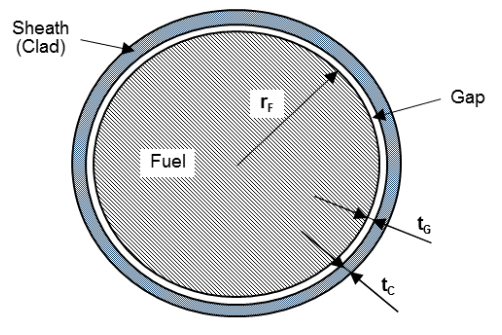
\includegraphics[width=0.7\linewidth]{figs/cylindrical fuel pin diagram.png}
    \caption{Cross section of a cylindrical Fuel Pin \cite{popov2017th}}
    \label{fig:fig_2}
\end{figure}

\begin{multicols}{2}

\begin{itemize}
    \item[] \textbf{Gap}

    Since there is no heat generation in the gap, therefore staedy-state conditions, Eqn. \ref{eq:4} transforms into the following equation:
    \begin{equation}\label{eq:13}
        {\frac{1}{r}}{\frac{d}{d r}}{\Bigg(}k_{g}r{\frac{d T}{d r}}{\Bigg)}=0
    \end{equation}
    
By integrating once,
\begin{equation}\label{eq:14}
    k_{g}r{\frac{d T}{d r}}=C
\end{equation}

The constant of integration is determined by considering the heat flux $q^{\prime \prime}$ at the fuel-gap
interface:
\begin{equation}\label{eq:15}
    -k_{g}\left[\frac{d T}{d r}\right]_{r=r_{F}}=q^{\prime \prime}=\frac{q^{\,\prime}}{2\pi r_{F}}\;
\end{equation}

Substituting Eqn. \ref{eq:15} into Eqn. \ref{eq:14} yields the following equation:
\begin{equation}\label{eq:16}
    k_{g}r\,\frac{d T}{d r}=-\frac{q^{\;\prime}}{2\pi}\Rightarrow k_{g}\,\frac{d T}{d r}=-\frac{q^{\;\prime}}{2\pi r}
\end{equation}

Assuming that the gap conductivity does not change significantly with temperature and performing integration, the temperature difference in the gap can be obtained as:
\begin{equation}\label{eq:17}
\begin{gathered}
        k_{g}\Delta T_{G A P}=k_{g}\left(T_{F}-T_{C}\right)= \\ {\frac{q^{\,\prime}}{2\pi}}\ln\left({\frac{r_{F}+t_{G}}{r_{F}}}\right)    
\end{gathered}
\end{equation}

The boundary condition, $T=T_C$ at $r=r_F+t_G$. Finally, the gap temperature difference is obtained as:
\begin{equation}\label{eq:18}
    \Delta T_{G A P}={\frac{q^{'}}{2\pi k_{G}}}\ln\left({\frac{r_{F}+t_{G}}{r_{F}}}\right)
\end{equation}

Since $t_g$ (gap thickness) is usually very small, we can expand the log term to write,
\begin{equation}\label{eq:19}
    \Delta T_{_{G A P}}=\frac{q}{2\mathcal{\pi}\,r_{F}}\biggl(\frac{t_{_G}}{k_{_G}}\biggr)
\end{equation}

After a period of operation the gap will contain a mixture of the original gas and fission product gases, hence the thermal conductivity $k_g$ will change over core life. Defining an effective coefficient of gap heat transfer $h_{gap}$ such that the temperature drop across the gap is:

\[\Delta T\Big|_{g a p}=-\frac{q^{\prime \prime}}{h_{g a p}}\]

The heat flux across the gap in steady state must be just the amount of heat produced in the fuel divided by the surface area of the fuel:

\[q^{\prime \prime}=-{\frac{q^{\prime \prime \prime}\left(\pi\,r_{f}^{2}\,\Delta T\right)}{2\pi\,r_{f}\,\Delta T}}\ \ ={\frac{q^{\prime \prime \prime}r_{f}}{2}}\ \ ={\frac{q^{\prime}}{2\pi r_{f}}}\]

By considering the above, the temperature difference in the gap can be obtained as follows:
\begin{equation}\label{eq:20}
    \Delta T_{G A P}=\frac{q^{\prime}}{2\pi r_{F}h_{G}}
\end{equation}

\item[] \textbf{Clad} 

The steady-state equation for the cladding region, in which there is no heat generation, is similar as gap region,

\[{\frac{1}{r}}{\frac{d}{d r}}{\Bigg(}k_{c}r{\frac{d T}{d r}}{\Bigg)}=0\]

This equation is solved in the same manner as for the gap to yield:
\begin{equation}\label{eq:21}
\begin{gathered}
        k_{c}\Delta T_{C L A D}=k_{c}\left(T_{c}-T_{s}\right) \\ =\frac{q^{\prime}}{2\pi}\ln\left(\frac{r_{F}+t_{G}+t_{C}}{r_{F}+t_{G}}\right) \\ \Rightarrow\;\Delta T_{C L A D}=\frac{q^{'}}{2\pi k_{c}}\ln\left(\frac{r_{F}+t_{G}+t_{C}}{r_{F}+t_{G}}\right)
\end{gathered}
\end{equation}

The subscript $S$ indicates the cladding-coolant surface interface. Since $t_g$ is very small then by ignoring it and with expanding the log we get clad temperature difference is,
\begin{equation}\label{eq:22}
    \Delta T_{\scriptscriptstyle C L A D}=\frac{q^{\;\prime}}{2\pi\left(r_{F}+t_{\scriptscriptstyle G}\right)}\bigg(\frac{t_{\scriptscriptstyle C}}{k_{\scriptscriptstyle C}}\bigg)
\end{equation}

\item[] \textbf{Coolant}

Newton’s law of cooling describes heat transfer from the clad surface to the coolant, 
\begin{equation}\label{eq:23}
    \begin{gathered}
        q^{\prime \prime} = h_{\scriptscriptstyle S} \left(T_{\scriptscriptstyle S} - T_{\scriptscriptstyle FL}\right) \\
        T_S - T_{FL} = \frac{q^{\prime \prime}}{h_S}
    \end{gathered}
\end{equation}

where, $T_{FL}$ is the bulk temperature of the coolant fluid. Hence, the temperature drop from the cladding surface to the bulk fluid temperature is:
\begin{equation}\label{eq:24}
    \Delta T_{C O O L}=\frac{q^{\prime}}{2\pi h_{_{S}}\left(r_{_{F}}+t_{_{C}}+t_{_{G}}\right)}
\end{equation}

By summing up Eqns. \ref{eq:12}, \ref{eq:20}, \ref{eq:22} and \ref{eq:24} the overall temperature difference between the fuel centreline and the bulk coolant can be obtained according to the following equation:
\begin{equation}\label{eq:25}
\begin{gathered}
        T_{_{0}}-T_{_{F L}}= \\ \frac{q^{\,\prime}}{2\pi}\Biggl(\frac{1}{2\overline{{{k}}}_{f}}+\frac{1}{h_{_G}r_{_F}}+\frac{t_{_G}+t_{_C}}{k_{_C}\left(r_{_F}+t_{_G}\right)} \\ + \frac{1}{h_{_{{_S}}}\left(r_{_F}+t_{_G}+t_{_C}\right)}\Biggr)
\end{gathered}
\end{equation}

The expression in brackets in Eqn. \ref{eq:25} is the thermal resistance across the fuel element:
\begin{equation}\label{eq:26}
\begin{gathered}
            R_{t h}=\left(\frac{1}{2\overline{{{k}}}_{f}}+\frac{1}{h_{G}r_{F}} +\frac{t_{G}+t_{c}}{k_{C}\left(r_{F}+t_{G}\right)} \\ +\frac{1}{h_{S}\left(r_{F}+t_{G}+t_{C}\right)}\right)
\end{gathered}
\end{equation}

Hence, the centreline fuel temperature is greater than the coolant temperature by an amount that depends on the amount of heat generated and on various resistances to heat flow.

\end{itemize}

Figure \ref{fig:fig_3} illustrates the radial temperature distribution across a fuel element for two linear power levels: 45 kW/m (full-power operation) and 15 kW/m (decay power after shutdown) \cite{popov2017th}. The highest temperature gradient occurs within the fuel pellet, exceeding 1400$^{\circ} C$ at full power, due to the low thermal conductivity of $(UO_{2})$. Despite its thinness, the fuel-cladding gap shows a notable temperature drop. In contrast, the cladding and coolant, being good heat conductors, exhibit minimal temperature differences.

\end{multicols}

\begin{figure}
    \centering
    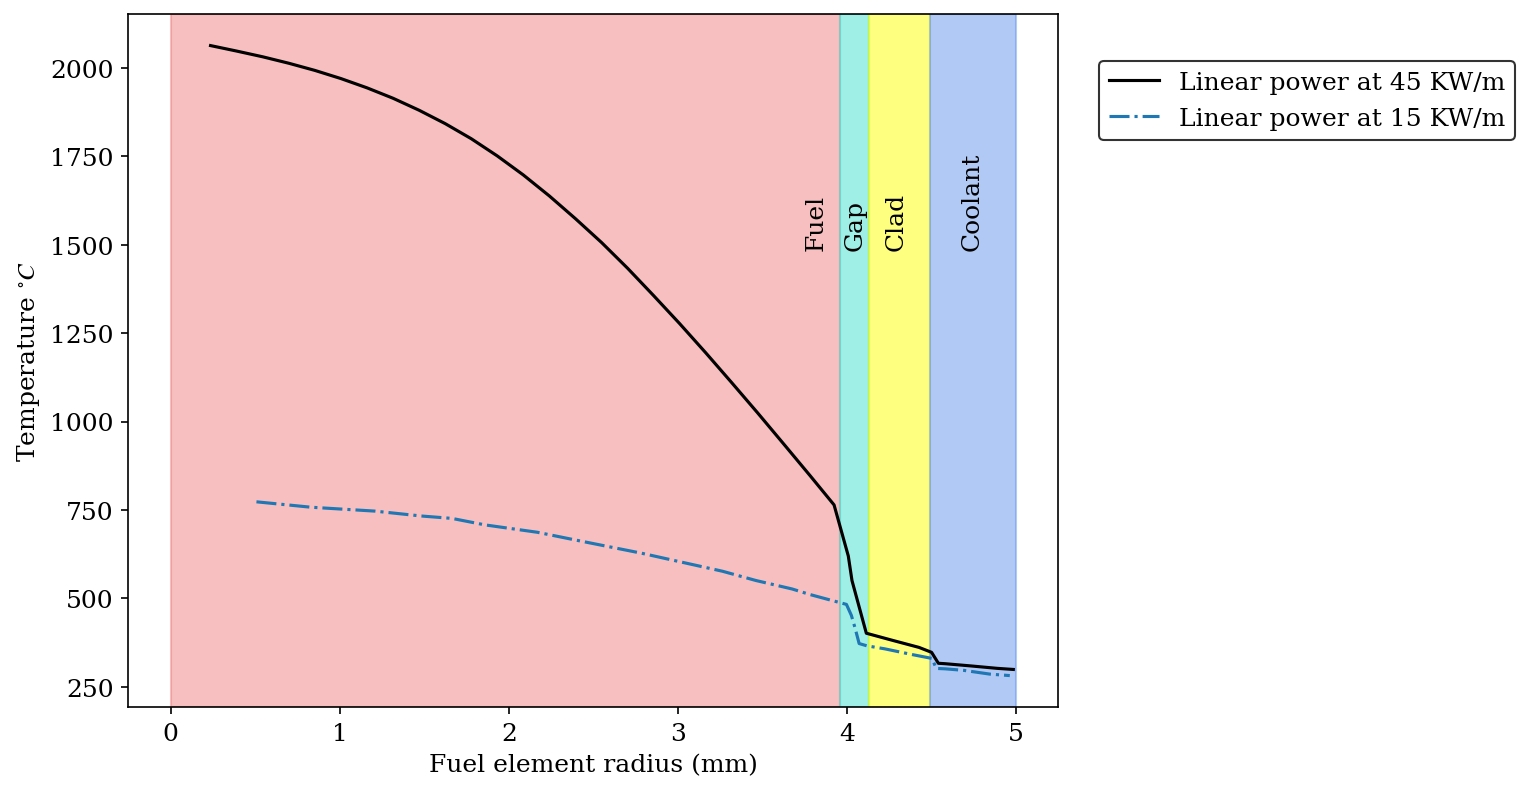
\includegraphics[width=0.8\linewidth]{figs/ass_2_temp_profile.png}
    \caption{Radial temperature distribution}
    \label{fig:fig_3}
\end{figure}

%%--------------------
%%  Numerical Methods
%%--------------------
\begin{multicols}{2}

\section{Numerical Methods}

\begin{enumerate}
    \item \textbf{Newton Iteration Process}

    To solve the steady-state radial heat conduction equation numerically, we can use the Newton Iteration Method to handle the nonlinearity introduced by temperature-dependent thermal conductivity. The governing equation for heat conduction in a cylindrical fuel element is given by:
    \begin{equation}\label{eq:27}
        \frac{1}{r}\frac{\partial}{\partial r}\!\left(r k\frac{\partial T}{\partial r}\right)\!+\!q^{\prime \prime \prime} = 0
    \end{equation}

    where $k(T)$ is the thermal conductivity, which varies with temperature. Using the finite difference method (FDM), the equation is discretized at a radial node $\textit{i}$ as:
    \begin{equation}\label{eq:28}
        \begin{split}
            \frac{1}{r_{i}} & \left[\frac{(r_{i+1}k_{i+1}T_{i+1}-r_{i}k_{i}T_{i})}{\Delta r^{2}} \right. \\ 
            & \left. -\frac{(r_{i}k_{i}T_{i}-r_{i-1}k_{i-1}T_{i-1})}{\Delta r^{2}}\right] 
            +q_{i}^{\prime \prime \prime}=0
        \end{split}
    \end{equation}

    Rearranging, the system of equations takes the form:
    \begin{equation}\label{eq:29}
        \begin{array}{c}
            a_{i-1}T_{i-1} + a_{i}T_{i} + a_{i+1}T_{i+1} = b_{i}, \\[8pt]
            a_{i-1} = \frac{r_{i-1}k_{i-1}}{r_{i}\Delta r^{2}}, \\[8pt]
            a_{i} = -\left(\frac{r_{i+1}k_{i+1} + r_{i-1}k_{i-1}}{r_{i}\Delta r^{2}}\right), \\[8pt]
            a_{i+1} = \frac{r_{i+1}k_{i+1}}{r_{i}\Delta r^{2}}, \quad 
            b_{i} = -q_{i}^{\prime \prime \prime}
        \end{array}
    \end{equation}

    To solve this nonlinear system, Newton’s iterative method is applied as follows:
    \begin{enumerate}
        \item Residual Function

        The residual at node $\textit{i}$ is given by:
        \[R_{i}(T)=a_{i-1}T_{i-1}+a_{i}T_{i}+a_{i+1}T_{i+1}-b_{i}\]

        \item Linearization Using Taylor Expansion

        Expanding $R_i(T)$ using first order Taylor series:
        \[R_{i}(T^{(n+1)})\approx R_{i}(T^{(n)})+\frac{\partial R_{i}}{\partial T}\Delta T=0\]

        \item Jacobian Matrix

    For each node $\textit{i}$:
    \begin{equation*}
        \begin{gathered}
            J_{i i}={\frac{\partial R_{i}}{\partial T_{i}}}=a_{i}+{\frac{d a_{i}}{d T}}T_{i} \\
            J_{i,i-1}=a_{i-1},\quad J_{i,i+1}=a_{i+1}
        \end{gathered}
    \end{equation*}

    \item Temperature Correction

    The Newton update equation is:
    \[J\Delta T=-R(T^{(n)})\]

    This system is solved using standard numerical solvers such as Gaussian elimination or LU decomposition method.

    \item Updating the Temperature Value

    The new temperature estimate is:
    \[T^{(n+1)}=T^{(n)}+\Delta T\]

    \item Convergence Check

    The iteration continues until the residual norm satisfies:
    \[\|R(T^{(n)})\|< \epsilon\]

    \end{enumerate}

    \item \textbf{Crank-Nicolson Method}

    To solve the transient radial heat conduction equation:
    \[\rho C p{\frac{\partial T}{\partial t}}={\frac{1}{r}}{\frac{\partial}{\partial r}}\bigg(r k{\frac{\partial T}{\partial r}}\bigg)+q^{\prime \prime \prime}\]

    we can use Crank-Nicolson Method, which is an implicit second-order time integration scheme.
    \begin{enumerate}
        \item Discretization

        Using finite difference grid with spatial nodes $\textit{i}$ and time steps $n$, the time derivative is approximated as:
        \begin{equation*}
            \begin{split}
                \frac{T_{i}^{n+1}-T_{i}^{n}}{\Delta t} &= \frac{1}{2} \Bigg[ 
            \left. \frac{1}{r} \frac{\partial}{\partial r} \left( r k \frac{\partial T}{\partial r} \right) \right|^{n+1} + \\  
            &\quad \left. \frac{1}{r} \frac{\partial}{\partial r} \left( r k \frac{\partial T}{\partial r} \right) \right|^{n} 
            \Bigg] + q_{i}^{\prime \prime \prime}
        \end{split}
    \end{equation*}

    Approximating the spatial derivative using the finite difference method (FDM):
    \begin{equation*}
        \begin{split}
            {\frac{1}{r_{i}}}{\frac{\partial}{\partial r}}\left(r k{\frac{\partial T}{\partial r}}\right) 
            & \\ \approx {\frac{1}{r_{i}}} \Bigg[
            \quad {\frac{r_{i+1}k_{i+1}(T_{i+1}-T_{i})}{\Delta r^{2}}} \\
            - {\frac{r_{i}k_{i}(T_{i}-T_{i-1})}{\Delta r^{2}}} \Bigg] 
        \end{split}
    \end{equation*}

    Applying this at both time steps $n$ and $n+1$, the Crank-Nicolson scheme results in a tridiagonal system of the form:
    \[A T^{n+1}=B T^{n}+b\]

    where $A$ and $B$ are tridiagonal matrices, and $b$ accounts for heat generation.

    \item Matrix Formulation

    For each node $i$, we get,
    \[a_{i-1}T_{i-1}^{n+1}+a_{i}T_{i}^{n+1}+a_{i+1}T_{i+1}^{n+1}=b_{i}\]

    Since the system is tridiagonal, we can solve for $T^{n+1}$ using iterative solver.

    \end{enumerate}

    \item \textbf{Computational Tools and Machine Learning Approaches}

    In addition to traditional numerical methods, commercial and open-source software packages are widely used for solving heat transfer and fluid flow problems in reactor cores. COMSOL Multiphysics, based on the Finite Element Method (FEM), is often employed for thermal analysis in complex geometries, providing flexibility in handling multi-physics interactions. ANSYS Fluent and OpenFOAM, both utilizing the Finite Volume Method (FVM), are extensively used for Computational Fluid Dynamics (CFD) simulations, particularly in modeling convective heat transfer in reactor coolant channels. For system-level thermal-hydraulic analysis, RELAP5, TRACE, and CATHENA are commonly used 1D system codes to simulate transient scenarios and safety analysis in nuclear reactors, incorporating empirical correlations and reduced-order modeling for efficient large-scale system simulations.

    Recently, Physics-Informed Neural Networks (PINNs) have emerged as a novel approach for solving fluid flow and heat conduction problems in reactor cores \cite{coppo2025application, jalili2024physics}. Unlike conventional numerical solvers that rely on discretization, PINNs leverage deep learning frameworks while embedding governing equations as constraints in the training process. This allows efficient surrogate modeling of heat transfer and turbulence phenomena, potentially accelerating transient simulations and providing real-time predictive capabilities.
    
\end{enumerate}

\end{multicols}

%%----------------------
%%    Conclusion
%%----------------------
\section{Conclusion}

The study of radial heat transfer in nuclear fuel elements is crucial for ensuring the thermal performance and safety of a reactor core. This assignment explored the fundamental heat transfer mechanisms, including conduction within the fuel and cladding, and convection in the coolant. The effects of material properties, power density, and burnup on radial heat transfer were discussed, highlighting the degradation of thermal conductivity over fuel life. Mathematical formulations were presented to describe steady-state and transient heat conduction, with numerical techniques such as the Newton iteration method and the Crank-Nicolson scheme used for solving these equations. Additionally, commercial and widely used system codes like RELAP5, TRACE, and CATHENA, along with computational tools such as COMSOL, ANSYS Fluent, and OpenFOAM, provide robust modeling capabilities for reactor thermal-hydraulics analysis. Emerging machine learning approaches, such as Physics-Informed Neural Networks, also show promise in enhancing predictive accuracy.

%--------------
%   Acronyms
%--------------

\section*{Acronyms}
\begin{acronym}[PINNs]
    \acro{FDM}{Finite Difference Method}
    \acro{FEM}{Finite Element Method}
    \acro{CFD}{Computational fluid dynamics}
    \acro{PINNs}{Physics-Informed Neural Networks}
\end{acronym}

%-----------------
% Bibliography
%-----------------

\bibliographystyle{IEEEtran} % You can choose a different style if needed
\bibliography{ref} % This refers to the Bibliography.bib file

\end{document}